\documentclass[11pt]{article}

\usepackage[a4paper,margin=20mm]{geometry}
\usepackage[T1]{fontenc}
\usepackage{lmodern}
\usepackage{microtype}
\usepackage{amsmath,amssymb,mathtools}
\usepackage{booktabs,array,tabularx}
\usepackage{siunitx}
\usepackage{tikz}
\usepackage{xcolor}
\usepackage[hidelinks]{hyperref}

\usetikzlibrary{positioning}

\definecolor{checkblue}{RGB}{0,79,128}
\definecolor{bitfill}{RGB}{235,244,250}
\definecolor{wrongorange}{RGB}{220,105,25}

\sisetup{
  detect-all,
  retain-explicit-plus,
  table-number-alignment=center
}

\newcommand{\Ncal}{\mathcal{N}}
\newcommand{\atanh}{\operatorname{atanh}}
\newcommand{\given}{\,\middle|\,}

\title{One Sum-Product Message-Passing Iteration\\
  for the Six-Bit, Two-Check Example}
\author{}
\date{}

\begin{document}
\maketitle
\vspace{-1.5em}

\begin{abstract}
This document gives every scalar used in one complete log-likelihood-ratio
(LLR) message-passing iteration for the six-bit example in \texttt{p2}.
It starts from the six displayed channel LLRs, forms all six
variable-to-check messages, evaluates the two check nodes for every recipient,
and combines the six check-to-variable messages into a-posteriori LLRs.
The numerical results are computed from the rounded LLRs printed in the source
slide; the extra decimal places below are computational precision, not extra
measurement precision.
\end{abstract}

\section{Graph, parity checks, and sign convention}

Bits are indexed from zero.  The parity-check matrix and the two parity-check
equations are
\begin{equation}
H=
\begin{bmatrix}
0&1&1&0&0&1\\
1&0&0&1&1&0
\end{bmatrix},
\qquad
\begin{aligned}
c_0 &: b_1\oplus b_2\oplus b_5=0,\\
c_1 &: b_0\oplus b_3\oplus b_4=0.
\end{aligned}
\label{eq:H}
\end{equation}
Thus \(\Ncal(c_0)=\{1,2,5\}\) and
\(\Ncal(c_1)=\{0,3,4\}\).  Every variable node has degree one, so this
cycle-free Tanner graph has two disconnected components, each containing one
check node.

\begin{figure}[htbp]
  \centering
  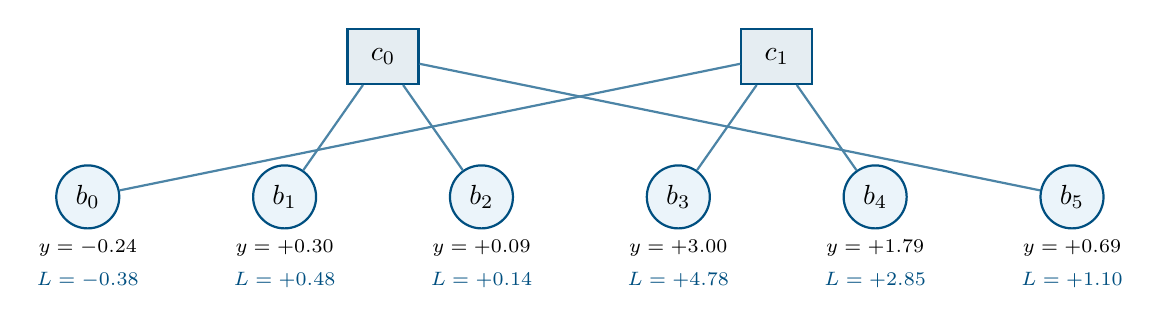
\begin{tikzpicture}[
    x=1.25cm,y=1.05cm,
    bit/.style={circle,draw=checkblue,fill=bitfill,line width=0.8pt,
      minimum size=8mm,inner sep=0pt},
    check/.style={rectangle,draw=checkblue,fill=checkblue!10,line width=0.8pt,
      minimum width=9mm,minimum height=7mm},
    edge/.style={draw=checkblue!70,line width=0.8pt}
  ]
    \node[check] (c0) at (-2,1.7) {$c_0$};
    \node[check] (c1) at ( 2,1.7) {$c_1$};

    \foreach \x/\i in {-5/0,-3/1,-1/2,1/3,3/4,5/5}
      \node[bit] (b\i) at (\x,0) {$b_{\i}$};

    \foreach \a/\b in {c0/b1,c0/b2,c0/b5,c1/b0,c1/b3,c1/b4}
      \draw[edge] (\a)--(\b);

    \foreach \x/\y/\ell in {
      -5/{-0.24}/{-0.38},-3/{+0.30}/{+0.48},-1/{+0.09}/{+0.14},
       1/{+3.00}/{+4.78}, 3/{+1.79}/{+2.85}, 5/{+0.69}/{+1.10}}
    {
      \node[font=\scriptsize] at (\x,-0.62) {$y=\y$};
      \node[font=\scriptsize,text=checkblue] at (\x,-1.00) {$L=\ell$};
    }
  \end{tikzpicture}
  \caption{The six variable nodes, the two check nodes, and the displayed
  observations and channel LLRs.}
  \label{fig:graph}
\end{figure}

The source example defines
\begin{equation}
L_i=\log\frac{P(b_i=1\mid y_i)}{P(b_i=0\mid y_i)},
\label{eq:llr-convention}
\end{equation}
so a positive LLR favours bit one.  With the bipolar mapping
\(x_i=2b_i-1\), bit one maps to \(+1\).  Each row of~\eqref{eq:H} requires its
three bits to have even parity and therefore satisfies
\(\prod_{i\in\Ncal(c)}x_i=-1\).  This target sign is why the check update in
Section~\ref{sec:check-update} has a leading minus sign.

The six observations \(y_i\) and six channel LLRs \(L_i\) are both treated as
given inputs.  The retained example does not specify the channel parameters
needed to derive the printed LLRs from the printed observations.

\section{Definition of one iteration}

One message-passing iteration using the flooding schedule is defined here as
the following three steps:
\begin{align}
U_{c\to i}^{(0)}&=0,
\label{eq:init}\\
Q_{i\to c}^{(1)}
  &=L_i+\sum_{a\in\Ncal(i)\setminus c}U_{a\to i}^{(0)},
\label{eq:variable-update}\\
U_{c\to i}^{(1)}
  &=-2\atanh\!\left(
    \prod_{j\in\Ncal(c)\setminus i}
    \tanh\!\frac{Q_{j\to c}^{(1)}}{2}
  \right),
\label{eq:check-update}\\
B_i^{(1)}
  &=L_i+\sum_{c\in\Ncal(i)}U_{c\to i}^{(1)}.
\label{eq:posterior-update}
\end{align}
Here \(Q_{i\to c}\) is a variable-to-check message,
\(U_{c\to i}\) is a check-to-variable message, and \(B_i^{(1)}\) is the
a-posteriori LLR after the iteration.  Because every variable has degree one,
the sum in \eqref{eq:variable-update} is empty and
\begin{equation}
Q_{i\to c}^{(1)}=L_i
\quad\text{on every edge.}
\label{eq:q-equals-l}
\end{equation}

\section{Inputs and variable-to-check messages}

Table~\ref{tab:inputs} contains the inputs, the initial hard decisions, and
every scalar entering the check-node calculations.  The initial hard decision
is \(\widehat b_i^{(0)}=\mathbb{1}[L_i\geq 0]\).

\begin{table}[htbp]
\centering
\small
\caption{Channel inputs and variable-to-check messages.}
\label{tab:inputs}
\begin{tabular}{
  c
  S[table-format=+1.2]
  S[table-format=+1.2]
  c c
  S[table-format=+1.2]
  S[table-format=+1.3]
  S[table-format=+1.9]
}
\toprule
{$i$} & {$y_i$} & {$L_i$} & {$\widehat b_i^{(0)}$} & {edge}
& {$Q_{i\to c}^{(1)}$} & {$Q/2$} & {$t_{i\to c}=\tanh(Q/2)$} \\
\midrule
0 & -0.24 & -0.38 & 0 & $0\to c_1$ & -0.38 & -0.190 & -0.187746206 \\
1 & +0.30 & +0.48 & 1 & $1\to c_0$ & +0.48 & +0.240 & +0.235495750 \\
2 & +0.09 & +0.14 & 1 & $2\to c_0$ & +0.14 & +0.070 & +0.069885890 \\
3 & +3.00 & +4.78 & 1 & $3\to c_1$ & +4.78 & +2.390 & +0.983347814 \\
4 & +1.79 & +2.85 & 1 & $4\to c_1$ & +2.85 & +1.425 & +0.890637366 \\
5 & +0.69 & +1.10 & 1 & $5\to c_0$ & +1.10 & +0.550 & +0.500520211 \\
\bottomrule
\end{tabular}
\end{table}

The transmitted word displayed in the source example is
\begin{equation}
\boldsymbol b=(0,1,0,1,1,1).
\end{equation}
Before message passing,
\begin{equation}
\widehat{\boldsymbol b}^{(0)}=(0,1,1,1,1,1),
\qquad
H\widehat{\boldsymbol b}^{(0)}\bmod 2=(1,0).
\label{eq:initial-syndrome}
\end{equation}
Only bit 2 is initially wrong, and only check \(c_0\) is violated.

\section{Check-to-variable messages}
\label{sec:check-update}

For compactness, define the product used to form the message from check \(c\)
to bit \(i\):
\begin{equation}
p_{c\to i}^{(1)}
=\prod_{j\in\Ncal(c)\setminus i}t_{j\to c}^{(1)}.
\end{equation}
Then \(U_{c\to i}^{(1)}=-2\atanh(p_{c\to i}^{(1)})\).  Each row of
Table~\ref{tab:check-messages} shows both transformed inputs, their product,
the inverse hyperbolic tangent, and the outgoing message.  The recipient's own
message is excluded from its row.

\begin{table}[htbp]
\centering
\scriptsize
\caption{Complete check-node arithmetic for every check-to-variable message.}
\label{tab:check-messages}
\setlength{\tabcolsep}{4.2pt}
\begin{tabular}{
  c c
  S[table-format=+1.9]
  S[table-format=+1.9]
  S[table-format=+1.9]
  S[table-format=+1.9]
  S[table-format=+1.9]
}
\toprule
{edge} & {other bits} & {$t_j$} & {$t_k$}
& {$p_{c\to i}^{(1)}$} & {$\atanh(p_{c\to i}^{(1)})$}
& {$U_{c\to i}^{(1)}$} \\
\midrule
$c_0\to1$ & $2,5$ & +0.069885890 & +0.500520211 & +0.034979301 & +0.034993577 & -0.069987155 \\
$c_0\to2$ & $1,5$ & +0.235495750 & +0.500520211 & +0.117870382 & +0.118420853 & -0.236841706 \\
$c_0\to5$ & $1,2$ & +0.235495750 & +0.069885890 & +0.016457830 & +0.016459316 & -0.032918633 \\
\addlinespace
$c_1\to0$ & $3,4$ & +0.983347814 & +0.890637366 & +0.875806306 & +1.357475742 & -2.714951483 \\
$c_1\to3$ & $0,4$ & -0.187746206 & +0.890637366 & -0.167213786 & -0.168798923 & +0.337597845 \\
$c_1\to4$ & $0,3$ & -0.187746206 & +0.983347814 & -0.184619821 & -0.186761347 & +0.373522694 \\
\bottomrule
\end{tabular}
\end{table}

For example, the reply from \(c_0\) to bit 2 excludes bit 2's own message:
\begin{align}
U_{c_0\to2}^{(1)}
&=-2\atanh\!\left[
  \tanh\!\left(\frac{Q_{1\to c_0}^{(1)}}{2}\right)
  \tanh\!\left(\frac{Q_{5\to c_0}^{(1)}}{2}\right)
  \right]\\
&=-2\atanh\!\left[
  \tanh(0.48/2)\tanh(1.10/2)
  \right]\\
&=-2\atanh(0.117870382293)\\
&=-0.236841705808.
\end{align}

\section{A-posteriori LLRs and decisions}

Because each variable node has degree one, each bit receives one
check-to-variable message, so \(B_i^{(1)}=L_i+U_{c\to i}^{(1)}\).  Under the
convention in \eqref{eq:llr-convention}, the posterior probability, the
posterior mean of \(x_i\), and the hard decision are
\begin{equation}
P_i^{(1)}=P(b_i=1\mid\boldsymbol y)
=\frac{1}{1+e^{-B_i^{(1)}}},
\qquad
\xi_i^{(1)}=\tanh\!\frac{B_i^{(1)}}{2},
\qquad
\widehat b_i^{(1)}=\mathbb{1}[B_i^{(1)}\geq0].
\label{eq:final-quantities}
\end{equation}

\begin{table}[htbp]
\centering
\small
\caption{Combination of the channel LLR and incoming check-to-variable message.}
\label{tab:posterior}
\setlength{\tabcolsep}{5.0pt}
\begin{tabular}{
  c
  S[table-format=+1.2]
  S[table-format=+1.9]
  S[table-format=+1.9]
  S[table-format=1.9]
  S[table-format=+1.9]
  c
}
\toprule
{$i$} & {$L_i$} & {incoming $U_{c\to i}^{(1)}$} & {$B_i^{(1)}$}
& {$P_i^{(1)}$} & {$\xi_i^{(1)}$} & {$\widehat b_i^{(1)}$} \\
\midrule
0 & -0.38 & -2.714951483 & -3.094951483 & 0.043315982 & -0.913368035 & 0 \\
1 & +0.48 & -0.069987155 & +0.410012845 & 0.601090959 & +0.202181918 & 1 \\
2 & +0.14 & -0.236841706 & -0.096841706 & 0.475808477 & -0.048383046 & 0 \\
3 & +4.78 & +0.337597845 & +5.117597845 & 0.994045276 & +0.988090551 & 1 \\
4 & +2.85 & +0.373522694 & +3.223522694 & 0.961709945 & +0.923419890 & 1 \\
5 & +1.10 & -0.032918633 & +1.067081367 & 0.744041476 & +0.488082953 & 1 \\
\bottomrule
\end{tabular}
\end{table}

The first message-passing iteration changes only bit 2:
\begin{equation}
\widehat{\boldsymbol b}^{(0)}=(0,1,1,1,1,1)
\quad\longrightarrow\quad
\widehat{\boldsymbol b}^{(1)}=(0,1,0,1,1,1).
\end{equation}
The resulting syndrome is
\begin{equation}
H\widehat{\boldsymbol b}^{(1)}\bmod 2=(0,0),
\end{equation}
so both parity checks are satisfied and the displayed transmitted word is
recovered.

Because the Tanner graph is cycle-free and each variable node has only one
check neighbour, this iteration already gives the exact bit marginals for the
six rounded channel LLRs.  Repeating the update does not change any message:
each variable-to-check message remains equal to its channel LLR.

\paragraph{Numerical provenance.}
The inputs and equations come from \texttt{os00\_exact\_example.tex}; the
retained checker is \texttt{exact\_six\_bit\_example.py}.  Every number in
Tables~\ref{tab:inputs}--\ref{tab:posterior} was independently recomputed from
the rounded channel LLRs.  Only sum-product quantities are included.

\end{document}
